\documentclass[a4paper]{article}
\usepackage[margin=20mm]{geometry}
\usepackage{amsmath,graphicx,booktabs}
\usepackage[hidelinks]{hyperref}

\title{Parallel Tempering and Iterated Local Search for Network Design}
\author{Quantum Icing Team}
\date{}

\begin{document}
\maketitle

\begin{abstract}
We combine parallel tempering and iterated local search on the QOBLIB \texttt{network24} instance, scoring each topology
by solving a continuous routing problem. A first parallel tempering run supplied a solution of 670,621.
Iterated local search reduced the objective to 661,760, and a second parallel tempering run reduced it to 657,121
in 62 seconds from that warm start. The verified integer objective is 0.989\% below the published reference of 663,688.
\end{abstract}

\section{Problem formulation}

The \texttt{network24} instance specifies traffic demands \(d_{sv}\) from source \(s\) to destination \(v\).
A topology is a set \(A\) of directed arcs, with two incoming and two outgoing arcs at each of the 24 vertices.
The \(24\cdot23=552\) binary link decisions therefore select exactly 48 arcs. The objective is to minimize the largest arc load.

For fixed \(A\), let \(f^s_{uv}\) be the amount of traffic from source \(s\) carried by arc \((u,v)\).
Demands are scaled by 1,000 to match the benchmark's units. The routing relaxation is
\begin{equation}
\label{eq:routing}
\begin{aligned}
z_{\mathrm{LP}}(A) = \min_{f,z}\;& z\\
\text{subject to}\quad
\sum_{u:(u,v)\in A} f^s_{uv} - \sum_{w:(v,w)\in A} f^s_{vw}
  &= 1{,}000\,d_{sv} && (s,\ v\ne s),\\
\sum_s f^s_{uv} &\le z && ((u,v)\in A),\\
f^s_{us}&=0 && ((u,s)\in A),\\
f^s_{uv}&\ge 0 && (s,\ (u,v)\in A).
\end{aligned}
\end{equation}
We solve \eqref{eq:routing} with HiGHS and use \(E(A)=z_{\mathrm{LP}}(A)\) as the search energy.
The benchmark requires integer flows, which we compute when a topology can improve the incumbent.

\section{Search methods}

\subsection{Parallel tempering}

Parallel tempering~\cite{hukushima1996} runs several replicas at fixed temperatures.
Each replica uses the Metropolis acceptance probability \(\min\{1,\exp[-(E'-E)/T]\}\) for a proposed change from \(E\) to \(E'\).
A high-temperature replica can more readily accept increases in congestion and leave a local minimum.
Exchanging configurations gives a low-temperature replica access to the topologies explored at higher temperatures.
The exchange probability for neighboring slots \(i,j\) is
\[
 p_{\mathrm{exchange}}=\min\!\left\{1,\exp\!\left[
 (T_i^{-1}-T_j^{-1})(E_i-E_j)\right]\right\}.
\]
Each round consists of 15 local steps followed by exchange attempts, alternating between the odd and even adjacent pairs.

A two-arc exchange replaces \((a,b),(c,d)\) with \((a,d),(c,b)\), preserving all degrees. We also rotate the heads
of three arcs and reverse directed triangles. The probabilities of drawing these move types were
77\%, 20\%, and 3\%, respectively, before rejection of self-loops and duplicate arcs. For exchanges and rotations,
half the draws for the first arc are uniform and half are weighted by the capacity duals from \eqref{eq:routing}.
Larger duals indicate arcs whose extra capacity would reduce the objective locally.

Solving a routing LP for every candidate would be expensive, so we first rank candidates by a bound on congestion.
Let \(h_A(s,v)\) be the directed shortest-path distance in hops. Every unit of demand from \(s\) to \(v\) contributes
at least \(h_A(s,v)\) units to the sum of arc loads. That sum is at most \(48z\), giving
\begin{equation}
\label{eq:bound}
 L(A)=\frac{1{,}000}{48}\sum_{s,v}d_{sv}\,h_A(s,v)\le z_{\mathrm{LP}}(A).
\end{equation}
Each step draws up to 60 candidates, with a 50\% probability of attempting a second move per candidate.
We retain the candidate with the smallest bound, skipping those with a cached LP value above \(E+3T\).
To implement the Metropolis test we draw \(U\) uniformly from \((0,1)\), which gives the acceptance threshold \(E-T\log U\).
If the bound \eqref{eq:bound} exceeds that threshold, the candidate is rejected.
Otherwise we use its cached LP value or solve \eqref{eq:routing}.
The biased proposal and Metropolis rule are used without a Hastings correction, yielding an optimization heuristic.

\subsection{Iterated local search}

Iterated local search (ILS) alternates a perturbation of the current topology with descent to a local minimum~\cite{lourenco}.
Our descent uses two-arc exchanges, reversals of directed cycles of length three or four, and swaps of two vertex labels.
For the label swap \(\pi\), each arc \((u,v)\) becomes \((\pi(u),\pi(v))\). The demand matrix stays fixed, so an unchanged
graph structure can yield a different routing objective.

Descent ranks the neighbors by a weighted version of \eqref{eq:bound}, replacing hop counts by weighted distances and
48 by the sum of the arc weights. It takes the first LP improvement and repeats.
To reduce solve time, ILS updates the routing LP in place and reuses the simplex basis of the parent topology.
Once descent stalls, perturbations of two to eight moves provide new starting points for descent.

The run also used an initial look-ahead from the shared starting topology. It scored neighbors within 1.5\% of the
starting objective, divided the ranked list among five chains, and ran descent from up to 12 such neighbors per chain.
This lets descent reach a lower objective by first visiting a neighbor with higher congestion.

\section{Computational results}

\begin{table}[htbp]
\centering
\caption{Checked objectives along the search that produced the submission. Times are measured from each run's start.}
\label{tab:runs}
\begin{tabular}{@{}lrrrr@{}}
\toprule
Run & Starting objective & Handoff or submission & Decrease & Time (s)\\
\midrule
PT r6    & 673,253 & 670,621 & 2,632 & 1,211\\
ILS run8 & 670,621 & 661,760 & 8,861 &   110\\
PT r7    & 661,760 & 657,121 & 4,639 &    62\\
\bottomrule
\end{tabular}
\end{table}

Table~\ref{tab:runs} and Figure~\ref{fig:progress} follow the topology passed from one run to the next.
The two PT runs used ten workers and ten geometrically spaced temperatures from 450 to 2,500. In each run the two
coldest slots started from the incumbent and the other eight from random routable topologies.

\begin{figure}[htbp]
\centering
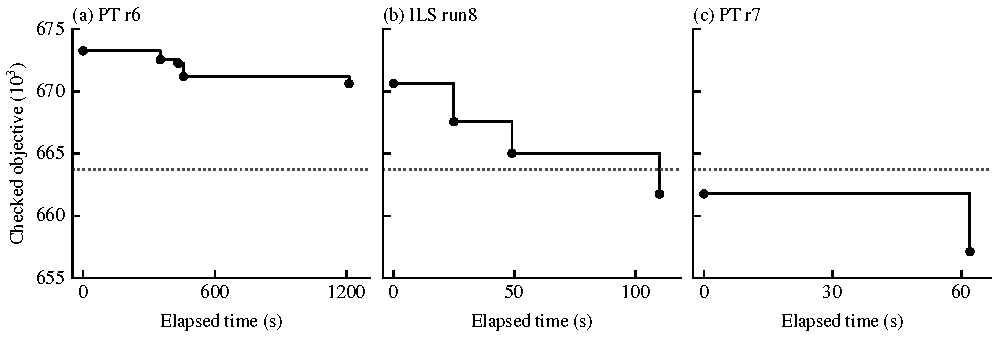
\includegraphics[width=\linewidth]{figures/pt-progress.pdf}
\caption{Checked objective along the PT--ILS--PT sequence. Each panel has its own time origin and ends at the
incumbent passed to the next stage or submitted. The dotted line is the QOBLIB reference.}
\label{fig:progress}
\end{figure}

Run r6 inherited the checked 673,253 topology from a preliminary PT run, r5, which started at 674,907.
Run r6 used seed 7 and a 30-minute budget. ILS took the 670,621 incumbent found at round 595,
while r6 was still running. All five ILS chains started from that topology and ran with a 20-minute budget.
During the initial look-ahead, the chain with seed 702 reached checked objectives of 667,560, 665,040, and 661,760.
A vertex-label swap during descent produced the last improvement, the first in this sequence below the QOBLIB reference
of 663,688~\cite{qoblib}.

\newpage
The second PT run, r7, used seed 8 and a 20-minute budget, starting from the ILS incumbent of 661,760.
In round 30, after 62 seconds, the coldest slot produced the submitted objective of 657,121, an improvement of
4,639 (0.701\%) from the ILS warm start and 6,567 (0.989\%) from the QOBLIB reference.
The incumbent stayed at 657,121 through round 597, when the run ended.

The local acceptance rate increased from 0.8\% at \(T=450\) to 33.8\% at \(T=2500\) (Figure~\ref{fig:diagnostics}).
The 544--659 pair accepted 2.7\% of its exchange attempts, while the 450--544 pair accepted 86.6\%.
The low acceptance across 544--659 indicates a bottleneck on this temperature ladder.

\begin{figure}[htbp]
\centering
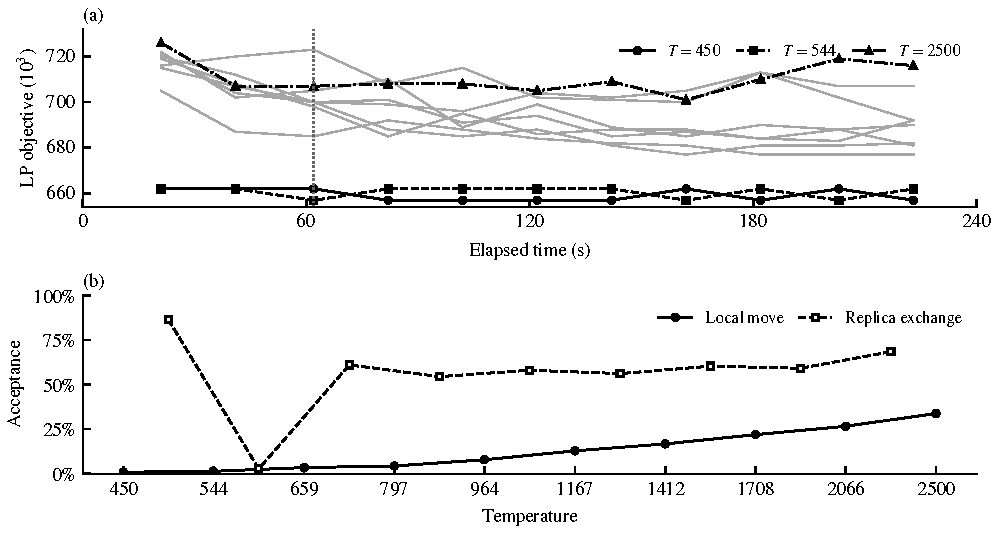
\includegraphics[width=\linewidth]{figures/pt-diagnostics.pdf}
\caption{Search dynamics in r7. (a) LP objective by temperature slot, sampled every ten rounds after exchanges and
rounded to the nearest thousand. The dotted line marks the verified improvement. (b) Cumulative acceptance rates
at round 597. Exchange rates are plotted at the geometric mean of each temperature pair.}
\label{fig:diagnostics}
\end{figure}

% \section{Verification and reproducibility}

% We re-solve \eqref{eq:routing} with integer variables when a candidate's LP bound permits an improvement.
% The referee checks the resulting \texttt{.sol} file before it replaces the incumbent.
% For the submitted topology, the LP gives \(657{,}120.967742\), so the verified maximum load of \(657{,}121\) is
% optimal for that topology. All computations were classical and used zero qubits.

% Verify the submitted file from the repository root with the Python environment active.
% \begin{verbatim}
% NETWORK_SOL_DIR=deliverables/network24 \
%   python network_pipeline.py status
% \end{verbatim}

% The traces come from \path{pt_r6.log}, \path{ils_run8.out}, and \path{pt_r7.log} under \path{ai_context/logs/}.
% The final topology is stored in \path{solutions/agent_pt/r7_best24.json}.
% The repository's \path{deliverables/README.md} gives the stage commands. Replaying the ILS and final PT stages
% from their historical starts would require recovering or regenerating the 670,621 and 661,760 topologies.

\begin{thebibliography}{9}
\bibitem{hukushima1996}
K. Hukushima and K. Nemoto.
\href{https://doi.org/10.1143/JPSJ.65.1604}{Exchange Monte Carlo method and application to spin glass simulations}.
\emph{Journal of the Physical Society of Japan}, 65(6), 1604--1608, 1996.

\bibitem{lourenco}
H. R. Lourenço, O. C. Martin, and T. Stützle.
\href{https://arxiv.org/abs/math/0102188}{Iterated local search}.
In \emph{Handbook of Metaheuristics}, pp.~320--353, 2003.

\bibitem{qoblib}
QOBLIB.
\href{https://github.com/ZIB-AOPT/QOBLIB/blob/main/08-network/solutions/README.md}{Network design benchmark, best-known values}.
\end{thebibliography}

\end{document}
